% EXP-004 Phase 2B manuscript — Natural Language Processing (Cambridge)
% Working draft; not submission-ready until authorship/declarations confirmed.
\documentclass[11pt,a4paper]{article}

\usepackage[margin=2.5cm]{geometry}
\usepackage{times}
\usepackage[T1]{fontenc}
\usepackage[utf8]{inputenc}
\usepackage{microtype}
\usepackage{amsmath,amssymb}
\usepackage{booktabs}
\usepackage{tabularx}
\usepackage{longtable}
\usepackage{multirow}
\usepackage{graphicx}
\usepackage{xcolor}
\usepackage{hyperref}
\usepackage{cleveref}
\usepackage{natbib}
\usepackage{setspace}
\usepackage{enumitem}
\usepackage{caption}
\usepackage{subcaption}
\usepackage{pgfplots}
\pgfplotsset{compat=1.18}
\usepackage{pgfplotstable}
\usepackage{siunitx}
\usepackage{csquotes}
\usepackage{url}

\hypersetup{
  colorlinks=true,
  linkcolor=black,
  citecolor=black,
  urlcolor=blue
}

\sisetup{round-mode=places,round-precision=2}

\title{Corpus Priming in Polish-to-Interslavic Translation with Large Language Models:\\
A Controlled Study Across Source Regimes}

\author{%
  Grzegorz R.\ Kulesza%
  \thanks{Corresponding author.
  Department of Medical Biophysics,
  Medical University of Bialystok, Bialystok, Poland.
  Email: \texttt{grzegorz.kulesza@umb.edu.pl}.
  Academic status (internal metadata): PhD / Assistant.}%
  \\[0.4em]
  \textit{Medical University of Bialystok}\\[0.6em]
  {\small\color{gray!60!black}
  % AUTHORSHIP PLACEHOLDER — do not treat as confirmed
  % [Potential coauthor pending confirmation: see AUTHORSHIP\_PENDING.md]
  }
}

\date{Working draft: 18 September 2026}

\begin{document}
\onehalfspacing
\maketitle

\begin{abstract}
Interslavic (ISV) is a constructed Slavic bridge language with limited digital resources relative to major national Slavic languages.
Large language models (LLMs) can be prompted to translate into ISV, but it remains unclear whether providing authentic ISV corpus material as context---\emph{corpus priming}---systematically shifts translation behaviour, and whether any such shift depends on thematic overlap between the source text and the priming corpus.
We report a controlled descriptive study of Polish-to-ISV translation under two conditions (Direct vs.\ Primed) across seven vendor model configurations, three independent repeats per cell, and three source regimes: HIGH (narrative, intentionally higher corpus overlap), LOW (narrative, lower overlap), and UNSEEN (shorter technical/expository voice-biophysics text from a domain absent from the priming corpus).
The primary metric is canonical ISV lexical coverage; the paired effect is $\Delta = \text{Primed} - \text{Direct}$.
Analysis is descriptive ($n{=}3$); no significance tests and no causal claims are made.
On a matched six-configuration comparison (excluding one invalid LOW pairing), mean $\Delta$ is $+7.39$ percentage points (pp) on HIGH, $+8.53$\,pp on LOW, and $+5.78$\,pp on UNSEEN.
Positive mean $\Delta$ is common but not universal: two Gemini configurations are negative on HIGH yet positive on LOW and UNSEEN.
Qualitative audits show that large HIGH gains often co-occur with corpus-opening motif reuse, whereas LOW and UNSEEN positives frequently involve lexical borrowing and orthographic cleanup without winter-narrative opening near-copy.
One Qwen LOW paired cell is invalid due to a Direct/Primed model-identity mismatch and is excluded from primary paired inference.
We conclude that authentic ISV corpus priming is associated with generally positive but strongly configuration-dependent coverage shifts that can persist under lower overlap and domain-unseen sources, without establishing that priming universally improves translation quality.
\end{abstract}

\noindent\textbf{Keywords:}
Interslavic;
machine translation;
large language models;
in-context learning;
low-resource languages

\tableofcontents
\newpage


\section{Introduction}
\label{sec:intro}

Machine translation (MT) into under-resourced target languages remains difficult even as neural and large-language-model (LLM) systems improve for high-resource pairs~\citep{koehn-knowles-2017-six,maillard-etal-2023-small}.
Interslavic (ISV; also Med\v{z}uslovjansky) is a constructed Slavic auxiliary language designed for mutual intelligibility across Slavic speech communities.
Relative to national Slavic languages with large web corpora and parallel datasets, ISV occupies a low-resource niche: usable dictionaries and community materials exist, but parallel Polish--ISV training data suitable for conventional neural MT are scarce, and automated evaluation infrastructure is not standardized in the same way as for WMT high-resource directions.

For Slavic speakers, Polish-to-ISV translation is practically interesting because Polish is a high-resource national language while ISV is intended as a bridge form.
For NLP methodology, the setting is interesting because it combines (i)~a target language with limited bitext, (ii)~available monolingual or curated target-side resources, and (iii)~commercial LLMs that can be prompted without gradient updates.
The methodological risk is equally clear: an attractive prompting trick can be mistaken for a validated translation method if experiments do not separate instruction-only behaviour from corpus-conditioned behaviour, and if they do not test whether apparent gains depend on thematic overlap between the source and the supplied corpus.

Prompting LLMs with instructions and in-context examples has become a practical route to translation without fine-tuning~\citep{brown2020language,hendy2023good,jiao2023chatgpt}.
A natural engineering idea for ISV is to place authentic ISV text in the prompt---here called \emph{corpus priming}---so that the model can condition generation on attested target-language material rather than on an instruction alone.
That idea is appealing, but it is not self-evidently beneficial.
Corpus material may encourage useful lexical and orthographic alignment; it may also encourage motif copying, register drift, or metric gains that do not correspond to communicative quality.
Moreover, if a source text already overlaps thematically with the priming corpus, apparent ``priming gains'' may partly reflect overlap rather than a generalizable priming intervention.

This paper reports EXP-004 Phase~2B: a controlled Polish-to-ISV study that separates Direct translation (no corpus) from Primed translation (authentic ISV corpus first, then translation), using identical model configurations, three independent repeats, and three source regimes that vary corpus overlap and genre:
\begin{itemize}[leftmargin=*]
  \item \textbf{HIGH}: narrative fiction deliberately inspired by the priming corpus;
  \item \textbf{LOW}: narrative fiction with intentionally weak thematic overlap;
  \item \textbf{UNSEEN}: shorter technical/expository educational text on human-voice biophysics, from a domain absent from the priming corpus registers.
\end{itemize}
The primary quantitative quantity is the paired difference in \emph{canonical ISV coverage}, $\Delta = \text{Primed}-\text{Direct}$.
Because each configuration cell has $n{=}3$ repeats, all quantitative reporting is descriptive: we do not perform significance testing and we do not claim causal identification of priming as a mechanism.

The study is deliberately comparative across regimes rather than optimized for a single leaderboard score.
HIGH asks whether priming is associated with coverage shifts when overlap is intentionally high.
LOW asks whether positive shifts can still appear when overlap is intentionally reduced.
UNSEEN asks whether positive shifts appear for a short technical/expository domain that is not represented in the narrative priming materials.
Together, the three regimes allow a restrained statement about persistence and heterogeneity without pretending that overlap, length, and genre have been orthogonally crossed.

\paragraph{Contributions.}
Conservatively stated, this paper contributes:
\begin{enumerate}[leftmargin=*]
  \item a reproducible Direct/Primed protocol for Polish-to-ISV LLM translation across seven configurations and three source regimes;
  \item a descriptive cross-regime evidence record for canonical coverage $\Delta$, including matched-configuration summaries and one documented invalid pairing cell;
  \item a qualitative paired audit synthesizing corpus-opening reuse, lexical borrowing, and orthographic change without equating metric gains with translation quality.
\end{enumerate}
We do \emph{not} claim that corpus priming universally improves translation, that higher overlap causes larger effects, or that any configuration is globally best.


\paragraph{Scope of claims.}
Throughout the paper we use associative language (``associated with'', ``observed'', ``descriptive'') rather than causal language (``improves'', ``causes'', ``proves''), except where we explicitly reject causal slogans.
This is not hedging for its own sake; it is required by the $n{=}3$ descriptive design and by the confounded regime factors.


\section{Related Work}
\label{sec:related}

\paragraph{LLM-based machine translation.}
LLMs can perform translation in zero- and few-shot settings without task-specific fine-tuning~\citep{brown2020language}.
Systematic evaluations report competitive quality for high-resource directions and weaker behaviour for low-resource pairs, with sensitivity to prompting strategy and domain~\citep{hendy2023good,jiao2023chatgpt,zhu2023multilingual}.
Document-level and domain-shift analyses further show that LLM translation behaviour is not a single scalar property of a model name: prompt packaging and domain can change outcomes~\citep{hendy2023good}.
Comparisons among GPT-family systems also illustrate that engine choice can dominate superficial ``ChatGPT vs.\ translator'' contrasts~\citep{jiao2023chatgpt}.
These findings motivate careful experimental design when the target language is under-resourced: gains observed under favourable prompting may not transfer across domains or source types.

A recurring methodological lesson in this literature is that prompting is itself an experimental factor.
Changing the presence, length, or identity of in-context material can move measured translation scores even when the underlying model family is held constant.
Our Direct vs.\ Primed contrast is intentionally narrow: it varies corpus presence while freezing the authentic corpus bytes and the source text within each regime.

\paragraph{Low-resource and multilingual MT.}
Data scarcity, domain mismatch, and rare-word behaviour remain core difficulties for neural MT~\citep{koehn-knowles-2017-six}.
Recent work continues to study how minimal or carefully selected data can still yield useful systems~\citep{maillard-etal-2023-small}.
Low-resource MT research often focuses on parallel-data collection, transfer learning, or multilingual training objectives.
Our setting differs: we do not train an NMT model on Polish--ISV bitext.
Instead we evaluate commercial/API LLM configurations under a fixed Direct vs.\ Primed prompting contrast.
This makes the work closer to an intervention study on prompting context than to a bitext-training bake-off.
The practical motivation remains related: when bitext is scarce, target-side authentic text may be the most available resource for conditioning generation.

\paragraph{In-context learning and example-based contextualization.}
Few-shot in-context learning~\citep{brown2020language} shows that providing demonstrations in the prompt can change task behaviour without weight updates.
Adaptive or example-conditioned LLM translation explores related ideas in which target-side or parallel material is supplied to guide generation~\citep{moslem2023adaptive}.
Multilingual LLM-MT analyses likewise emphasize that in-context examples and language coverage interact~\citep{zhu2023multilingual}.
Our \emph{corpus priming} condition supplies a frozen authentic ISV multi-register corpus before the translation request.
It is therefore related to in-context conditioning, but it is not a classical $k$-shot bitext demonstration protocol, nor a fine-tuning method.
The distinction matters for interpretation: a positive $\Delta$ indicates an association between corpus-conditioned prompting and the coverage metric, not proof that the model acquired a new grammar from the corpus.

\paragraph{Evaluation of translation and low-resource systems.}
Surface $n$-gram metrics such as BLEU~\citep{papineni-etal-2002-bleu} and learned metrics such as COMET~\citep{rei-etal-2020-comet} are widely used for MT evaluation; LLMs have also been studied as quality estimators~\citep{kocmi-federmann-2023-large}.
Each family of metrics encodes assumptions about references, human ratings, or learned representations that may not hold for Interslavic.
For ISV, we do not treat BLEU/COMET as primary endpoints in this experiment.
Phase~2B uses a project-specific resource-supported coverage stack (canonical coverage, broader coverage, unresolved rate, and orthography outside-inventory), designed around available ISV lexical/orthographic resources.
We explicitly warn that coverage is not a complete proxy for translation quality (\Cref{sec:evaluation}).
In low-resource settings, mismatched evaluation choices can create false confidence; we therefore keep metric language operational and separate qualitative audits from coverage tables.

\paragraph{Interslavic language technology.}
Interslavic is a community-developed Slavic auxiliary language with published grammars, dictionaries, and educational materials.
Computational work on Slavic NLP is extensive for national languages, but peer-reviewed evaluations of Polish-to-ISV LLM translation under controlled corpus priming remain scarce.
We therefore treat ISV primarily through operational definitions in this repository experiment rather than through a large prior MT literature.
Additional language-description citations suitable for a camera-ready related-work paragraph are listed in \texttt{REFERENCES\_NEEDED.md} when full bibliographic verification is still pending.

\paragraph{Positioning of this study.}
Relative to LLM-MT evaluations that sweep many language pairs, this paper is narrow and deep: one source language, one constructed target, three source regimes, seven configurations, and paired repeats.
Relative to purely anecdotal prompting notes, it is comparatively strict: frozen hashes, integrity gates, invalid-cell documentation, and an evidence map from claims to artifacts.
That trade-off is intentional for an under-resourced target where over-claiming would be especially costly.

\section{Research Questions}
\label{sec:rq}

We organize the study around six empirical questions.
They are answered descriptively from the Phase~2B evidence pack; none is treated as rhetorically settled in advance.

\begin{description}[style=nextline,leftmargin=1.2cm,font=\normalfont\bfseries]
  \item[RQ1] Does authentic ISV corpus priming produce a measurable shift in Polish-to-ISV translation outputs under the canonical coverage metric?
  \item[RQ2] Does this shift persist when the source text has lower thematic overlap with the priming corpus (LOW)?
  \item[RQ3] Does a positive paired shift persist for a domain-unseen, technical/expository source (UNSEEN)?
  \item[RQ4] How heterogeneous are priming effects across the seven model configurations?
  \item[RQ5] What qualitative textual changes accompany positive or negative shifts in canonical coverage?
  \item[RQ6] Which observed changes appear related to corpus-opening copying, lexical adoption, or orthographic normalization?
\end{description}

RQ1--RQ3 address magnitude and direction of $\Delta$ across regimes.
RQ4 addresses configuration dependence.
RQ5--RQ6 connect metric movement to audited textual behaviour without asserting causal mechanisms.


The RQs are ordered from measurement (RQ1) through generalization across sources (RQ2--RQ3) to heterogeneity and mechanism-facing description (RQ4--RQ6).
This order mirrors the analysis workflow actually used in the repository: regime aggregates first, then combined synthesis, then qualitative audits.

\section{Experimental Design}
\label{sec:design}

\subsection{Conditions}
Each translation session is assigned to one of two conditions:

\begin{itemize}[leftmargin=*]
  \item \textbf{Direct}: the model receives the Polish source and a translation instruction into Interslavic, without the authentic priming corpus.
  \item \textbf{Primed}: the model first receives the frozen authentic ISV corpus, then the translation instruction and Polish source.
\end{itemize}

The corpus is never shortened for any configuration.
For Gemini Primed runs, corpus delivery uses a recorded multi-message protocol (corpus in message~1; translation request in message~2) because of interface/context-window constraints (\Cref{sec:repro}).
All other scientific factors---source text, configuration identity, and repeat structure---are held as constant as the collection interfaces allow.

\subsection{Pairing and effect definition}
For each configuration and replicate $i\in\{\mathrm{r01},\mathrm{r02},\mathrm{r03}\}$,
\[
\Delta_i = C(\mathrm{Primed}_i) - C(\mathrm{Direct}_i),
\]
where $C$ denotes canonical ISV coverage (reported as a percentage; $\Delta$ in percentage points).
Configuration-level summaries use the mean of the three replicate $\Delta_i$ values.
All comparisons are descriptive.
The paired construction is the reason a Direct/Primed model-identity mismatch invalidates a cell: $\Delta$ is not defined as a same-model priming effect unless both sides share the intended configuration.

\subsection{Factorial structure}
Within each source regime the planned design is:
\[
7\ \text{configurations}\ \times\ 2\ \text{conditions}\ \times\ 3\ \text{repeats}\ =\ 42\ \text{runs}.
\]
Repeats are independent fresh sessions.
The same seven configurations are used in HIGH, LOW, and UNSEEN.
Across the full Phase~2B programme this yields $3\times 42=126$ planned runs, of which one LOW paired configuration is invalid for priming inference.

\subsection{Why the analysis is descriptive}
With $n{=}3$ per configuration cell, the study is not powered for inferential claims about population effects.
We report means, standard deviations, ranges, and sign consistency.
We do not compute $p$-values, confidence intervals intended for inferential generalization, or model rankings.
This is a deliberate epistemological choice aligned with the sample size, not an accidental omission.

\begin{table}[t]
\centering
\caption{Experimental design and source regimes (Phase~2B).}
\label{tab:design}
\begin{tabular}{@{}llp{5.6cm}@{}}
\toprule
\textbf{Regime} & \textbf{Source (frozen v1)} & \textbf{Design notes} \\
\midrule
HIGH & \emph{Iskra i Wieloryb\ldots} (30\,061\,B) & Narrative; intentionally higher corpus overlap \\
LOW & \emph{Podk\l{}ady} (15\,249\,B) & Narrative; intentionally lower overlap \\
UNSEEN & \emph{\'{C}wiczenie 2.2 --- Biofizyka g\l{}osu\ldots} (5\,676\,B) & Expository technical; domain unseen \\
\midrule
\multicolumn{3}{@{}p{0.92\linewidth}@{}}{\footnotesize
Conditions: Direct vs.\ Primed.
Configurations: 7.
Repeats: 3 independent sessions.
Planned runs per regime: 42.
Effect: $\Delta=\text{Primed}-\text{Direct}$ (canonical coverage, descriptive).
Priming corpus: \texttt{phase2a-authentic-isv} v1 (SHA-256 \texttt{aaad28e4\ldots a857}), never shortened.} \\
\bottomrule
\end{tabular}
\end{table}


\subsection{Operator protocol notes}
Runs were collected as independent sessions following the Phase~2B kits prepared for each regime.
Intake verification checked completeness and identity metadata before evaluation.
Analysis scripts aggregate already-evaluated runs and do not call LLMs.
These process controls do not eliminate vendor stochasticity, but they make the Direct/Primed pairing auditable after the fact.

\section{Corpus and Source Regimes}
\label{sec:corpus}

\subsection{Authentic priming corpus}
All Primed runs use the frozen authentic three-register corpus \texttt{phase2a-authentic-isv} v1
(SHA-256 \texttt{aaad28e43935a40313585d77a33bfc788d97e8d69b081f9486af74d52ca1a857}).
The corpus is held constant across regimes and configurations.
It is never shortened, paraphrased, or filtered to evade interface constraints.
Prior corpus self-evaluation under the same evaluator stack provides a reference ceiling for reading coverage magnitudes; it is not a translation baseline and is not used as a Direct/Primed control.

Keeping the corpus fixed is essential for the scientific contrast: regime differences are differences in the Polish source (and associated genre/length/overlap properties), not silent edits to the priming material.

\subsection{Source regimes}
\Cref{tab:design} summarizes the three regimes.
Length and genre differ jointly with overlap by design.

\paragraph{HIGH.}
Frozen Polish narrative \emph{Iskra i Wieloryb --- wersja z oryginalnymi nazwami} v1
(SHA-256 \texttt{ab8a0dcf7352789c09c4aca132c086999c861407e4cd682ee9414aab5b792f63}; 30\,061 bytes / 440 lines).
Classification: \texttt{high\_overlap\_corpus\_inspired}.
The story deliberately shares motifs with the priming corpus (for example winter narrative material associated with the corpus register excerpt used in qualitative opening checks).
HIGH is therefore not an ``independent same-topic'' control; it is the high-overlap arm of the design.

\paragraph{LOW.}
Frozen Polish narrative \emph{Podk\l{}ady} v1
(SHA-256 \texttt{ce1c4fca03fe9cb2c5f8181ab45c91767759a0c785f0a066543d95bc32f5271b}; 15\,249 bytes / 141 lines).
Classification: \texttt{low\_overlap}.
Contemporary municipal/archive plot with intentionally weak thematic overlap with the priming corpus and with the HIGH story.
Clean-prose boundary decisions (exclusion of casting notes and unrelated preamble material) were operator-approved before freeze.

\paragraph{UNSEEN.}
Frozen Polish educational theory text \emph{\'{C}wiczenie 2.2 --- Biofizyka g\l{}osu ludzkiego} v1
(SHA-256 \texttt{cd3bfb9a819b415e3cfb382e0737ba22540ccb679d0d34983c40dfbf89a9f7f4}; 5\,676 bytes after validation hash basis).
Classification: \texttt{unseen\_domain}.
Voice/speech biophysics exposition; domain absent from HIGH/LOW narrative registers and from the priming corpus domains under the project's validation record.
Exact bibliographic provenance of the teaching-derived source is incompletely known and is disclosed as a limitation.

\paragraph{Design confounds (disclosed).}
Overlap, length, and genre are not orthogonally crossed.
UNSEEN is shorter and expository; HIGH/LOW are longer narratives.
Magnitude comparisons across regimes are therefore descriptive and must not be read as causal attributions to overlap alone.
The manuscript treats these differences as first-class design characteristics rather than as nuisances to be narrated away after seeing the results.


\subsection{Why three regimes rather than one}
A single-regime study could not separate high-overlap narrative behaviour from lower-overlap or domain-unseen behaviour.
Three regimes increase confounds (length/genre) but buy interpretive breadth: persistence of positive $\Delta$ under LOW and UNSEEN cannot be dismissed as merely HIGH-overlap artefact, while HIGH still documents that negatives are possible even when overlap is intentional.

\section{Models and Experimental Conditions}
\label{sec:models}

We evaluate seven Phase~2B configurations, named exactly as in the canonical experiment artifacts (\Cref{tab:models}).
Configurations differ by vendor model and, where applicable, thinking/mode switches exposed by the interface used for collection.
No configuration is treated as a gold standard.

\begin{table}[t]
\centering
\caption{Model configurations evaluated in all three regimes (canonical labels).}
\label{tab:models}
\begin{tabular}{@{}ll@{}}
\toprule
\textbf{Short label} & \textbf{Canonical configuration name} \\
\midrule
Gemini ON & Gemini 3.6 Flash --- extended thinking ON \\
Gemini OFF & Gemini 3.6 Flash --- extended thinking OFF \\
Claude Sonnet 5 & Claude Sonnet 5 --- Medium (default) \\
DeepSeek Expert ON & DeepSeek V3 Expert --- DeepThink ON \\
Qwen 3.8 Max Fast & Qwen 3.8 Max --- Fast \\
GPT-5.6 Luna & GPT-5.6 Luna --- thinking OFF \\
Grok 4.5 Fast & Grok 4.5 Fast \\
\bottomrule
\end{tabular}
\end{table}


\paragraph{Gemini ON vs.\ OFF.}
Two Gemini 3.6 Flash configurations differ only in the extended-thinking switch (ON vs.\ OFF).
Both use the multi-message Primed protocol described in \Cref{sec:repro}.

\paragraph{What is held constant.}
Within a regime, all configurations translate the same frozen Polish source under the same Direct/Primed definitions, with three independent repeats.
Cross-regime comparisons reuse the same configuration list.

\paragraph{What is not claimed.}
Vendor display names and mode switches are operational labels for reproducibility.
We do not equate interface labels with internal model checkpoints beyond what the operator interfaces exposed at collection time, and we do not rank configurations by quality.


\subsection{Collection interfaces as part of the method}
Because the experiment uses vendor chat/API surfaces rather than a single open-weights checkpoint under identical decoding controls, configuration identity includes the operator-facing mode switches recorded at collection time.
That is a feature of the ecological validity of the study and a limitation for mechanistic attribution to a specific open checkpoint.
The manuscript therefore reports configuration labels exactly and avoids rewriting them into unofficial synonyms.


\subsection{Non-goals of the configuration set}
The seven configurations were chosen as representative Phase~2B operator-facing setups, not as an exhaustive survey of all vendors or decoding hyperparameters.
Absence of an open-weights local baseline is a limitation for mechanistic replication, not an accidental omission in the Results tables.

\section{Evaluation Methodology}
\label{sec:evaluation}

\subsection{Primary and secondary metrics}
Each completed run is scored with the project's deterministic ISV evaluation stack implemented in \texttt{src/isv\_eval/} (CLI entry via the project's \texttt{isv-eval} tooling).
Scoring does not call an LLM.
The metrics used in Phase~2B are:

\begin{itemize}[leftmargin=*]
  \item \textbf{canonical coverage} (primary): share of lexical tokens classified as resource-supported under the canonical inventory policy;
  \item \textbf{broader resource-supported coverage}: canonical-supported tokens plus additional lexical tokens with qualifying exact attestation in audited alternative resources;
  \item \textbf{unresolved rate}: share of lexical tokens in the unresolved (unsupported) bucket;
  \item \textbf{orthography outside-inventory}: character-level count of letters/symbols outside the accepted Interslavic Latin inventory (separate diagnostic in \texttt{src/isv\_eval/orthography.py}).
\end{itemize}

Manuscript quantitative claims focus on canonical coverage and its paired $\Delta$.
Other metrics are retained in the machine-readable datasets for audit and are not collapsed into a single composite score.
In particular, unresolved rate tends to move inversely with canonical coverage under the evaluator construction; reporting both without inventing a composite avoids double-counting the same inventory phenomenon under two names.

\subsection{Operational definition of canonical coverage}
The evaluator tokenizes model output and distinguishes \emph{lexical} (word-like) tokens from non-lexical tokens (punctuation, numbers, and similar).
Coverage denominators use lexical tokens only, as documented in the metrics module denominator policy.

\paragraph{Token and lookup policy.}
A token is treated as lexical when it contains at least one Unicode letter (\texttt{src/isv\_eval/normalize.py}).
Surface forms are not rewritten for display; normalization builds lookup keys only (NFC + lowercase; an optional secondary folded key for selected etymological characters).
Cyrillic tokens may be transliterated to Latin for lookup by the morphology backend.
Each lexical token is classified into inventory buckets used by the metrics module (\texttt{src/isv\_eval/metrics.py}, \texttt{classifier.py}, \texttt{lexicon.py}):
bucket~A (exact dictionary match), bucket~B (morphologically justified under available ISV resources), or bucket~C (unresolved).
Canonical coverage is $(A+B)/\text{lexical\_tokens}$.
Broader coverage additionally counts selected unresolved tokens that carry exact alternative-resource attestation; the broader tier is an evidence estimate, not a validity claim.

\paragraph{Orthography diagnostic.}
Orthography outside-inventory counts characters outside the accepted Interslavic Latin inventory (standard letters, etymological extensions, and sanctioned alternatives documented in the orthography module).
Polish-specific letters absent from that inventory (e.g.\ \emph{\k{a}}, \emph{\l{}}, \emph{\'{o}}, \emph{\.{z}}) are flagged when present.
The orthography check never repairs text and never enters the coverage denominators.

\paragraph{Implementation location.}
Metric definitions and denominator policy are implemented in \texttt{src/isv\_eval/metrics.py}; character audit in \texttt{src/isv\_eval/orthography.py}; Phase~2B aggregates regenerate from per-run \texttt{evaluation.json} / \texttt{orthography.json} via \texttt{scripts/analyze\_exp004\_phase2b.py}.

\subsection{What coverage is not}
Canonical coverage is a screening metric for resource-supported ISV lexical realization.
It is \emph{not} claimed to be equivalent to:
\begin{itemize}[leftmargin=*]
  \item human-judged translation quality,
  \item adequacy/fluency in the sense of DA/MQM protocols,
  \item BLEU~\citep{papineni-etal-2002-bleu} or COMET~\citep{rei-etal-2020-comet}.
\end{itemize}
Orthographic cleanup or substitution of inventory-supported synonyms can move coverage without implying a global quality improvement.
Conversely, communicative improvements that do not increase inventory hits may be invisible to the metric.
This asymmetry is why the paper pairs every major quantitative claim with qualitative audits and explicit limitations.

\subsection{Paired analysis unit}
The experimental unit for priming effects is the Direct$\leftrightarrow$Primed pair within a configuration and replicate, not an unpaired mixture of runs.
Configuration summaries average three paired $\Delta_i$ values.
Invalid pairs are excluded from primary paired inference rather than imputed.

\subsection{Qualitative audit}
For each regime, all valid Direct$\leftrightarrow$Primed pairs were inspected in a descriptive qualitative audit (HIGH and UNSEEN: 21 pairs; LOW primary: 18 valid pairs).
Audits record apparent classes such as lexical borrowing, orthographic cleanup, corpus-opening alignment, and degradations, without adjudicating full linguistic correctness.
Opening-overlap checks against a corpus narrative excerpt are used as an operational detector for winter-opening near-copy, especially to contrast HIGH against LOW/UNSEEN.

\subsection{Reporting conventions used in Results}
Unless otherwise stated, coverage means are percentages averaged over three Direct or three Primed runs, and $\Delta$ means are averages of three paired differences.
We report two decimal places in percentage points when that precision is present in the combined tables.
Sign consistency is reported as all-positive, all-negative, or mixed within the three replicates.
Invalid cells are marked explicitly rather than imputed.

\section{Results}
\label{sec:results}

All quantitative results below reconstruct from the canonical combined synthesis and the underlying HIGH/LOW/UNSEEN analysis artifacts.
No numbers were re-estimated for this manuscript.
Where we round to two decimal places in percentage points, rounding follows the combined evidence tables and does not change sign or qualitative interpretation.

\subsection{Integrity and validity}
HIGH and UNSEEN each collected and evaluated 42/42 planned runs with seven valid paired configurations (21 pairs).
LOW collected 42/42 retained runs but has six valid paired configurations (18 pairs) because the Qwen cell is \texttt{INVALID --- MODEL MISMATCH} (\Cref{sec:repro}).
Integrity gates (unique run IDs; complete Direct$\leftrightarrow$Primed pairing structure) pass on all three regimes.
These integrity facts are prerequisites for interpreting any mean $\Delta$: a missing or mismatched pair would silently break the Direct/Primed contrast.

\subsection{Central configuration-level $\Delta$ table}
\Cref{tab:deltas} is the primary quantitative table for later discussion and for RQ1--RQ4.
Reading the table by columns emphasizes regime behaviour; reading by rows emphasizes configuration heterogeneity.
Both views are necessary.
A column-only summary would hide Gemini's HIGH negatives; a row-only focus on one ``successful'' configuration would hide attenuation and invalid cells elsewhere.

\begin{table}[t]
\centering
\caption{Central cross-regime configuration mean $\Delta$ (canonical coverage, percentage points).
LOW Qwen cell is invalid and shown as ---.}
\label{tab:deltas}
\begin{tabular}{@{}lrrr@{}}
\toprule
\textbf{Configuration} & \textbf{HIGH $\Delta$} & \textbf{LOW $\Delta$} & \textbf{UNSEEN $\Delta$} \\
\midrule
Gemini ON & $-0.55$ & $+13.23$ & $+5.68$ \\
Gemini OFF & $-1.75$ & $+10.40$ & $+6.09$ \\
Claude Sonnet 5 & $+14.28$ & $+12.11$ & $+6.42$ \\
DeepSeek Expert ON & $+9.25$ & $+6.19$ & $+3.83$ \\
Qwen 3.8 Max Fast & $+5.18$ & --- & $+3.52$ \\
GPT-5.6 Luna & $+8.62$ & $+5.31$ & $+5.52$ \\
Grok 4.5 Fast & $+14.49$ & $+3.95$ & $+7.12$ \\
\bottomrule
\end{tabular}
\begin{flushleft}
\footnotesize
Source: \texttt{experiments/exp004-modelscreen/phase2b/analysis/combined/cross\_regime\_table.csv}.
Each cell is the mean of three replicate $\Delta_i$ values except LOW Qwen (invalid model mismatch).
\end{flushleft}
\end{table}


\subsection{Direct and Primed means}
In addition to $\Delta$, \Cref{tab:dpmeans} reports configuration-level Direct and Primed mean coverage.
This table clarifies whether a positive $\Delta$ arises from a large Primed gain, a low Direct baseline, or both.
For example, Gemini LOW combines comparatively low Direct means with substantially higher Primed means, whereas several HIGH positives combine mid Direct means with Primed means above 80\%.
Absolute Direct/Primed levels should be read separately from $\Delta$: a large positive $\Delta$ can arise from a low Direct baseline, a high Primed ceiling, or both, and absolute coverage remains a screening metric rather than a quality score.
\begin{table}[t]
\centering
\caption{Direct and Primed mean canonical coverage (\%) by configuration and regime.
LOW Qwen paired means are omitted (invalid).}
\label{tab:dpmeans}
\scriptsize
\begin{tabular}{@{}lrrrrrr@{}}
\toprule
 & \multicolumn{2}{c}{\textbf{HIGH}} & \multicolumn{2}{c}{\textbf{LOW}} & \multicolumn{2}{c}{\textbf{UNSEEN}} \\
\cmidrule(lr){2-3}\cmidrule(lr){4-5}\cmidrule(lr){6-7}
\textbf{Config.} & D & P & D & P & D & P \\
\midrule
Gemini ON & 68.68 & 68.13 & 64.33 & 77.56 & 65.77 & 71.45 \\
Gemini OFF & 67.20 & 65.45 & 64.51 & 74.91 & 63.85 & 69.95 \\
Claude & 69.29 & 83.57 & 65.72 & 77.83 & 66.07 & 72.48 \\
DeepSeek & 74.53 & 83.78 & 68.93 & 75.12 & 67.97 & 71.80 \\
Qwen & 76.36 & 81.54 & --- & --- & 67.65 & 71.17 \\
GPT-5.6 & 73.54 & 82.16 & 70.75 & 76.06 & 68.53 & 74.05 \\
Grok & 68.35 & 82.84 & 69.32 & 73.27 & 65.90 & 73.02 \\
\bottomrule
\end{tabular}
\begin{flushleft}
\footnotesize
Source: \texttt{analysis/combined/analysis.json} / \texttt{cross\_regime\_table\_full.csv}
(machine-readable; preferred over rounded prose tables).
\end{flushleft}
\end{table}



\subsection{All-configuration vs.\ matched-six summaries}
Unequal all-configuration means must not be treated as a matched three-regime average:

\begin{itemize}[leftmargin=*]
  \item HIGH: mean of 7 configuration $\Delta$s $= +7.07$\,pp (5 positive, 2 negative);
  \item LOW: mean of 6 valid configuration $\Delta$s $= +8.53$\,pp (6 positive);
  \item UNSEEN: mean of 7 configuration $\Delta$s $= +5.45$\,pp (7 positive).
\end{itemize}

For direct cross-regime comparison we use the matched six configurations available in all regimes (\Cref{tab:matched}):
HIGH $+7.39$\,pp, LOW $+8.53$\,pp, UNSEEN $+5.78$\,pp.
The matched-six construction excludes Qwen because LOW cannot supply a valid same-model paired effect for that configuration.
This exclusion is a validity decision, not a performance ranking.

\begin{table}[t]
\centering
\caption{Matched-six regime summary (identical six configurations on HIGH/LOW/UNSEEN; Qwen excluded).}
\label{tab:matched}
\begin{tabular}{@{}lrr@{}}
\toprule
\textbf{Regime} & \textbf{Mean $\Delta$ (pp)} & \textbf{$n$ configs} \\
\midrule
HIGH & $+7.39$ & 6 \\
LOW & $+8.53$ & 6 \\
UNSEEN & $+5.78$ & 6 \\
\bottomrule
\end{tabular}
\begin{flushleft}
\footnotesize
Included: Gemini ON, Gemini OFF, Claude Sonnet 5, DeepSeek Expert ON, GPT-5.6 Luna, Grok 4.5 Fast.
Descriptive only; not a statistical test.
\end{flushleft}
\end{table}


\subsection{Replicate consistency}
Sign consistency of the three replicate $\Delta_i$ values varies by configuration and regime (\Cref{fig:replicates}):
\begin{itemize}[leftmargin=*]
  \item HIGH: Gemini ON/OFF and Qwen show mixed signs; Claude, DeepSeek, GPT, and Grok are all-positive.
  \item LOW (valid): five configurations are all-positive; Grok is mixed (one negative replicate).
  \item UNSEEN: all 21 replicate $\Delta$s are positive.
\end{itemize}
Particularly variable HIGH cells include Grok (SD$(\Delta)\approx 5.90$\,pp) and Qwen (SD$(\Delta)\approx 5.56$\,pp).
More stable examples include GPT on HIGH (SD$(\Delta)\approx 1.34$\,pp) and Claude/DeepSeek on UNSEEN (SD$(\Delta)\approx 1.11$ / $1.06$\,pp).
Variance is reported as a descriptive property of the sample, not as a formal test of equality of variances.

\begin{figure}[t]
\centering
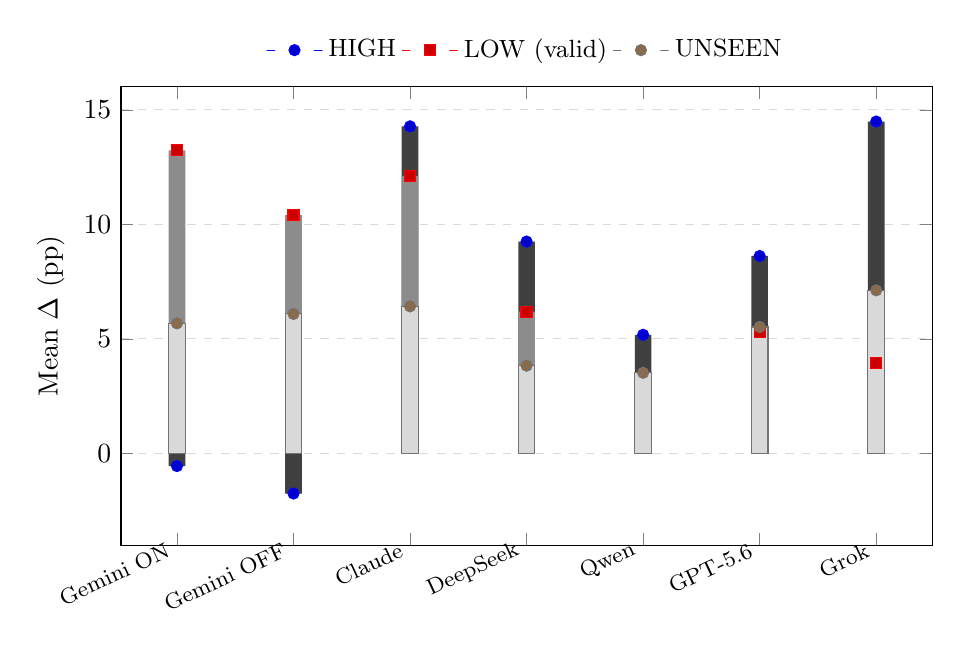
\begin{tikzpicture}
\begin{axis}[
  width=0.98\linewidth,
  height=7.4cm,
  ymajorgrids=true,
  grid style={dashed,gray!30},
  ylabel={Mean $\Delta$ (pp)},
  symbolic x coords={Gemini ON,Gemini OFF,Claude,DeepSeek,Qwen,GPT-5.6,Grok},
  xtick=data,
  x tick label style={rotate=25,anchor=east,font=\footnotesize},
  legend style={at={(0.5,1.03)},anchor=south,legend columns=3,font=\small,draw=none},
  ymin=-4, ymax=16,
  enlarge x limits=0.08,
  bar width=6pt,
]
\addplot+[ybar, fill=black!75, draw=none] coordinates {
  (Gemini ON,-0.55) (Gemini OFF,-1.75) (Claude,14.28) (DeepSeek,9.25)
  (Qwen,5.18) (GPT-5.6,8.62) (Grok,14.49)
};
\addplot+[ybar, fill=black!45, draw=none] coordinates {
  (Gemini ON,13.23) (Gemini OFF,10.40) (Claude,12.11) (DeepSeek,6.19)
  (GPT-5.6,5.31) (Grok,3.95)
};
\addplot+[ybar, fill=black!15, draw=black!55] coordinates {
  (Gemini ON,5.68) (Gemini OFF,6.09) (Claude,6.42) (DeepSeek,3.83)
  (Qwen,3.52) (GPT-5.6,5.52) (Grok,7.12)
};
\legend{HIGH,LOW (valid),UNSEEN}
\end{axis}
\end{tikzpicture}
\caption{Configuration-level mean canonical-coverage $\Delta$ across regimes.
LOW omits Qwen (invalid Direct/Primed model mismatch).
Descriptive only; no inferential intervals.}
\label{fig:configdeltas}
\end{figure}

\begin{figure}[t]
\centering
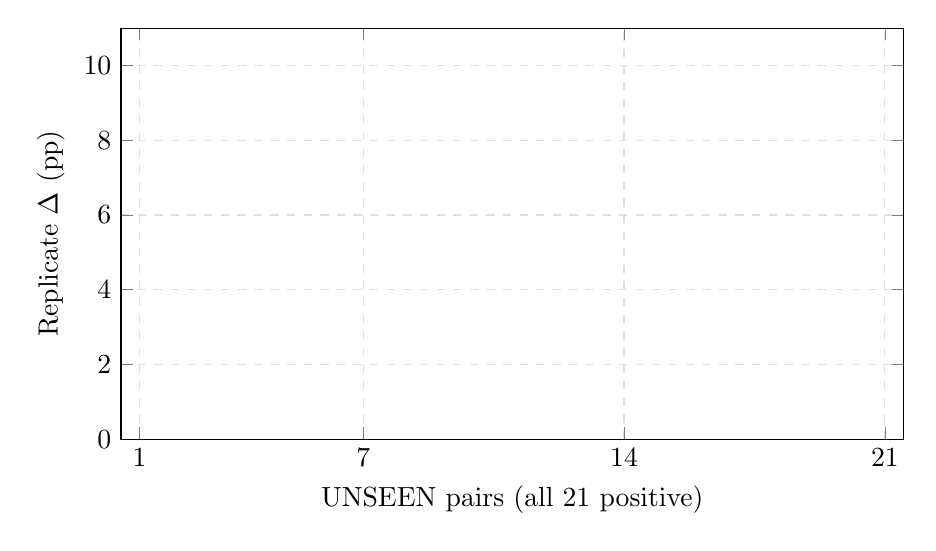
\begin{tikzpicture}
\begin{axis}[
  width=0.95\linewidth,
  height=6.8cm,
  ylabel={Replicate $\Delta$ (pp)},
  xlabel={UNSEEN pairs (all 21 positive)},
  only marks,
  mark size=2.2pt,
  ymin=0, ymax=11,
  xmin=0.5, xmax=21.5,
  xtick={1,7,14,21},
  grid=major,
  grid style={dashed,gray!25},
]
% All 21 UNSEEN replicate deltas from combined analysis (config order)
\addplot[black] coordinates {
  (1,2.12) (2,6.08) (3,8.84)
  (4,7.97) (5,3.96) (6,6.35)
  (7,7.14) (8,5.14) (9,6.96)
  (10,2.91) (11,5.00) (12,3.58)
  (13,3.67) (14,1.27) (15,5.62)
  (16,6.56) (17,7.58) (18,2.43)
  (19,6.02) (20,9.62) (21,5.70)
};
\addplot[gray,dashed,forget plot] coordinates {(0.5,0) (21.5,0)};
\end{axis}
\end{tikzpicture}
\caption{UNSEEN replicate-level paired $\Delta$ values (canonical coverage).
All 21 Direct$\leftrightarrow$Primed pairs are positive.
Points are ordered by configuration (Gemini ON, Gemini OFF, Claude, DeepSeek, Qwen, GPT-5.6 Luna, Grok), three replicates each.
Descriptive display only.}
\label{fig:replicates}
\end{figure}


\subsection{Regime-level reading of the metric}
On HIGH, mean $\Delta$ spans a wide range: from $-1.75$\,pp (Gemini OFF) to $+14.49$\,pp (Grok).
On LOW, valid means are all positive and Gemini becomes strongly positive.
On UNSEEN, means are moderate and uniformly signed at both configuration and replicate levels.
These patterns answer different questions: HIGH shows that priming is not uniformly helpful under the metric even when overlap is high; LOW and UNSEEN show that positive associations are not confined to high-overlap narrative material.

\subsection{Answering RQ1--RQ3 at the metric level}
RQ1: priming is associated with measurable $\Delta$ shifts, but not with a single universal sign on HIGH.
RQ2: on LOW, every \emph{valid} configuration mean $\Delta$ is positive; Gemini means are large ($+13.23$ / $+10.40$\,pp).
RQ3: on UNSEEN, every configuration mean $\Delta$ is positive and every replicate $\Delta$ is positive.
These statements are descriptive coverage observations, not quality or causality claims.


\subsection{Configuration-level commentary (descriptive)}
The following comments restate \Cref{tab:deltas} in prose so that later Discussion can refer to patterns without reintroducing numbers from memory.

\paragraph{Gemini.}
Both Gemini configurations have negative mean $\Delta$ on HIGH ($-0.55$ and $-1.75$\,pp) with mixed replicate signs.
On LOW they become the largest valid positives ($+13.23$ and $+10.40$\,pp), all replicates positive.
On UNSEEN they remain positive ($+5.68$ and $+6.09$\,pp), all replicates positive.
This is the clearest cross-regime reversal in the study.

\paragraph{Claude Sonnet 5.}
Claude is positive in every regime mean and every replicate in the primary tables.
Magnitudes are large on HIGH/LOW and smaller on UNSEEN.
The pattern is persistence with attenuation toward the short technical source, not a sign flip.

\paragraph{DeepSeek Expert ON.}
DeepSeek is likewise persistently positive, with a smooth attenuation sequence $+9.25\rightarrow +6.19\rightarrow +3.83$\,pp.
Among valid configurations, it is one of the clearest monotonic magnitude declines across the three regimes.

\paragraph{Qwen 3.8 Max Fast.}
Qwen contributes valid positive means on HIGH ($+5.18$\,pp, mixed replicates) and UNSEEN ($+3.52$\,pp, all positive).
LOW remains invalid; therefore Qwen cannot enter matched-six summaries.

\paragraph{GPT-5.6 Luna.}
GPT is positive everywhere in the primary means, with relatively stable HIGH replicates and similar LOW/UNSEEN magnitudes.
It is an example of a moderate, persistent association rather than an extreme HIGH-only spike.

\paragraph{Grok 4.5 Fast.}
Grok shows a large HIGH mean ($+14.49$\,pp), a much smaller LOW mean ($+3.95$\,pp) with one negative replicate, and a positive UNSEEN mean ($+7.12$\,pp).
The scientific point is magnitude instability across regimes, not a claim that Grok is ``best'' or ``worst.''

\section{Qualitative Analysis}
\label{sec:qual}

This section synthesizes the regime qualitative audits and the combined qualitative synthesis.
Examples are traceable to audited configuration/replicate cells; no invented illustrations are used.
The audit language is intentionally cautious: labels such as ``lexical borrowing'' or ``improvement'' are apparent classes relative to orthographic/resource signals and corpus-overlap observations, not adjudicated proof of linguistic correctness.

\subsection{Corpus-opening and motif copying}
On HIGH, large positive $\Delta$ cells often co-occur with primed openings that track the authentic corpus winter narrative (audit cue: \emph{Ljudi govoret, \v{z}e v tamtoj denj\ldots}).
Documented examples include Claude HIGH (mean $\Delta +14.28$\,pp) and DeepSeek HIGH (mean $\Delta +9.25$\,pp), where Kit$\rightarrow$Velryb and corpus lexis such as \emph{pomalo}, \emph{jedino}, \emph{\v{c}r\v{e}z} appear with opening alignment.
Qwen HIGH r01--r02 show opening adoption with positive $\Delta$, while r03 is negative despite opening presence---a reminder that opening copy is not sufficient for a positive metric shift.

On LOW, primed openings remain recognizably \emph{Podk\l{}ady} (Katarzyna/Katarina + archive).
Opening Jaccard against the winter corpus excerpt stays low (maximum $\approx 0.09$ in the LOW audit).
Nevertheless, Gemini LOW shows large positive mean $\Delta$ without systematic winter-opening near-copy.
This contrast is one of the strongest qualitative results in the study: the textual signature that accompanies many HIGH positives is largely absent from LOW positives.

On UNSEEN, primed texts open with exercise/biophysics titles (e.g.\ \emph{Vje\v{z}ba}/\emph{Upra\v{z}nenje} + \emph{Biofizika \ldots glasa}), not the winter story; opening Jaccard remains low for all 21 pairs.
If corpus priming ``worked'' only by transplanting the winter narrative, UNSEEN positives should not occur in this form.

\subsection{Lexical borrowing and orthographic cleanup}
Across regimes, primed outputs frequently show corpus-register lexical items (\emph{\v{c}r\v{e}z}, \emph{jedino}, \emph{govoret}, \emph{pomalo}, \emph{no} for Polish \emph{ale}) while retaining source plot or expository structure.
Concrete LOW example: Gemini ON r01, $\Delta +15.84$\,pp, with \emph{\v{c}r\v{e}z}/\emph{govoret} and no winter-opening rewrite.
Orthographic / Polish-residue reductions often co-occur with positive $\Delta$ (e.g.\ LOW Claude r01, outside-inventory $301\rightarrow 11$ with $\Delta +13.82$\,pp; HIGH Claude r01, $365\rightarrow 18$), but dimensions can diverge (coverage down with ortho up, or both up).
Therefore orthographic cleanup is best described as a recurrent correlate, not as a sufficient explanation of $\Delta$.

\subsection{Positive $\Delta$ without obvious corpus-opening copying}
LOW Gemini ON/OFF cell means ($+13.23$ / $+10.40$\,pp) and UNSEEN Gemini ON r03 ($+8.84$\,pp) illustrate positive coverage shifts with little or no winter-motif transplant.
UNSEEN Qwen r02 ($+1.27$\,pp) shows the complementary pattern: markers may be present without a large coverage move.
These cases are central to RQ6: metric-positive priming is compatible with lexical/orthographic calibration rather than wholesale narrative copying, and surface corpus cues are not a reliable thermometer of $\Delta$ magnitude.

\subsection{Structural and domain preservation}
LOW primed outputs keep the urban/archive plot; UNSEEN keeps educational biophysics terminology (\emph{formant*}, \emph{rezonan*}, \emph{biofizik*}) in both Direct and Primed.
Title/name churn occurs (HIGH whale-title variants; LOW Katarina/Katarzyna; UNSEEN exercise-title variants) and should not be equated with priming success.
Markdown or formatting artifacts can also appear (e.g.\ UNSEEN GPT primed r03 title formatting) without invalidating run completeness under the project's intake rules; such surface noise is another reason not to equate coverage with polished quality.

\subsection{RQ5 summary}
Positive coverage shifts are accompanied by heterogeneous textual changes: HIGH often shows opening/motif alignment plus lexical adoption; LOW/UNSEEN more often show lexical and orthographic shifts inside preserved source structure.
Negative or mixed HIGH Gemini cells show reshuffles without reliable corpus-opening adoption and sometimes show rising Polish-residue or outside-inventory signals.
The qualitative layer therefore supports configuration- and regime-dependent descriptions rather than a single Primed ``style.''

\section{Cross-Regime Analysis}
\label{sec:cross}

\subsection{Overall direction}
Matched-six means are positive in all three regimes (\Cref{tab:matched}).
UNSEEN adds a uniformly positive replicate pattern (21/21) on a short technical source.
LOW shows that large positive $\Delta$ can appear under intentionally low thematic overlap.
HIGH is the only regime with negative configuration mean $\Delta$ (both Gemini conditions).
Taken together, the regimes support a tempered summary: positive associations are common across regimes, but HIGH shows that common is not universal at the configuration level.

\subsection{Configuration-specific patterns}
We characterize heterogeneity without ranking:

\begin{itemize}[leftmargin=*]
  \item \textbf{Gemini ON/OFF:} negative or near-zero mean $\Delta$ on HIGH with mixed replicates; strongly positive on LOW; moderately positive on UNSEEN. This is a clear HIGH$\rightarrow$LOW direction reversal.
  \item \textbf{Claude Sonnet 5:} positive mean $\Delta$ in all three regimes; HIGH/LOW large; UNSEEN smaller ($+6.42$\,pp).
  \item \textbf{DeepSeek Expert ON:} persistently positive with attenuation HIGH$\rightarrow$LOW$\rightarrow$UNSEEN ($+9.25\rightarrow +6.19\rightarrow +3.83$\,pp).
  \item \textbf{GPT-5.6 Luna:} persistently positive; HIGH larger than LOW/UNSEEN, which are similar ($+5.31$ / $+5.52$\,pp).
  \item \textbf{Grok 4.5 Fast:} large positive HIGH; much smaller LOW mean with one negative replicate; positive UNSEEN.
  \item \textbf{Qwen 3.8 Max Fast:} positive HIGH and UNSEEN means; no valid LOW paired effect.
\end{itemize}

These patterns differ in kind, not merely in rank order.
Reversal (Gemini), attenuation (DeepSeek), magnitude instability without mean-sign flip (Grok), and missing cells (Qwen LOW) are distinct descriptive phenomena.

\subsection{Overlap is not a sufficient explanation}
If larger overlap were necessary for positive priming $\Delta$, LOW and UNSEEN should not show widespread positives.
They do.
Gemini's largest positives appear on LOW rather than HIGH.
Overlap, length, and genre remain confounded, so these observations reject a simple ``overlap causes $\Delta$'' slogan without identifying an alternative single cause.
A responsible scientific statement is therefore comparative and negative with respect to that slogan: high overlap is not required for positive coverage $\Delta$ in this design.

\subsection{Length and genre as disclosed confounds}
UNSEEN's smaller matched-six mean ($+5.78$\,pp) should not be narrated as ``weaker priming because the domain is unseen'' without acknowledging that UNSEEN is also shorter and expository.
Likewise, HIGH's mixture of large positives and Gemini negatives cannot be attributed solely to overlap.
The cross-regime section therefore prioritizes pattern description over monocausal storytelling.

\subsection{RQ4}
Configuration heterogeneity is first-order: sign reversals, attenuation, amplification, and invalid cells coexist in the same experimental frame.
Collapsing the study into a single universal priming effect would misrepresent the evidence.

\subsection{Practical reading for manuscript users}
For readers who need a one-paragraph takeaway without collapsing heterogeneity, the safest summary is:
matched-six mean $\Delta$ is positive in HIGH, LOW, and UNSEEN; UNSEEN replicate $\Delta$s are uniformly positive; HIGH uniquely contains negative Gemini means; LOW uniquely lacks a valid Qwen paired estimate; qualitative audits show that HIGH positives often involve opening reuse while LOW/UNSEEN positives often do not.
Any shorter slogan loses at least one of those facts.

\section{What the Qualitative Evidence Suggests About Mechanisms}
\label{sec:mechanisms}

We discuss mechanisms cautiously as hypotheses constrained by audits, not as proven causal pathways.
The goal is to connect RQ5--RQ6 to the quantitative tables without over-fitting a single story to every configuration.

\paragraph{Hypothesis A: lexical/register calibration.}
Priming may increase the density of corpus-consistent ISV lexical choices and reduce Polish-residue forms, moving canonical coverage without rewriting source structure.
LOW and UNSEEN positives with retained plot/exposition are compatible with this hypothesis.
Under this view, the corpus functions less as a narrative template and more as a register/lexicon prior exposed in context.

\paragraph{Hypothesis B: orthographic normalization.}
Outside-inventory reductions often co-occur with positive $\Delta$, suggesting that orthographic cleanup is one pathway by which the metric can move.
Divergent cases show it is neither necessary nor sufficient.
Metric--ortho divergence is itself scientifically useful: it warns against treating any single diagnostic as a complete account of Primed behaviour.

\paragraph{Hypothesis C: corpus-opening reuse under high overlap.}
On HIGH, large positives recurrently co-occur with winter-opening near-copy in the qualitative audit.
This may inflate coverage when corpus lexis enters the output, but it is not the only route to positive $\Delta$, and opening copy can appear with negative $\Delta$ (Qwen HIGH r03).
Hypothesis~C therefore explains a HIGH-local signature rather than the whole experiment.

\paragraph{Compatibility, not competition.}
A, B, and C are not mutually exclusive.
A configuration can show orthographic cleanup and lexical borrowing; a HIGH run can show opening reuse plus lexical adoption.
The important empirical constraint is that A/B-compatible behaviour on LOW/UNSEEN indicates that opening-copy (Hypothesis~C) is not necessary for observing a positive coverage $\Delta$.

\paragraph{What we do not claim.}
We do not claim that models ``learned Interslavic'' from the corpus in a demonstrated causal sense, that priming is the sole cause of $\Delta$, or that metric gains equal communicative quality.
A useful descriptive framing---not a formal law---is that priming appears to be a \emph{context-sensitive intervention} whose observed effect depends on the interaction between model configuration and source regime.

\paragraph{Consequences for future experiments.}
If Hypothesis~C dominates in a future high-overlap narrative arm, experiments should measure opening overlap explicitly rather than treating it as anecdotal.
If Hypotheses~A/B dominate in low-overlap or unseen arms, evaluation should track lexical inventory hits and orthography separately from narrative similarity.
Phase~2B already separates those diagnostics; future designs can pre-register which diagnostic is primary for which regime.

\section{Reproducibility and Operational Findings}
\label{sec:repro}

\subsection{Qwen LOW invalid pairing}
For LOW Qwen 3.8 Max --- Fast, Direct runs used the intended model, but Primed runs were executed with \textbf{Qwen3.7-Plus} (default-selected in the chat interface).
The paired cell is therefore \texttt{INVALID --- MODEL MISMATCH}.
Any historical numerical $\Delta$ for that cell (including $-12.08$\,pp) must not be interpreted as a Qwen 3.8 Max LOW priming effect.
A later attempt to run the intended Qwen3.8-Max Primed condition encountered a service/security block; no corpus-shortening or prompt-evasion workaround was performed.
Outputs were retained with validity sidecars.
Incident record: \texttt{experiments/exp004-modelscreen/phase2b/analysis/low/QWEN\_INCIDENT.md}.

\subsection{Gemini multi-message Primed protocol}
Gemini Primed runs deliver the full corpus in message~1 and the translation request in message~2.
Corpus bytes are not shortened.
This is a recorded interface/context-window constraint applied consistently across regimes, not a redesign of the priming material.

\subsection{Artifact provenance}
Canonical experiment root: \texttt{experiments/exp004-modelscreen/phase2b/}.
Final synthesis: \texttt{analysis/combined/}.
Historical checkpoint files that predate UNSEEN completion are not used as the current experimental state for manuscript claims.


\subsection{Replication package expectations}
A reader seeking to regenerate the quantitative tables should start from the regime analysis JSON files and the combined synthesis, not from historical checkpoint prose.
The manuscript's \texttt{EVIDENCE\_MAP.md} lists stable paths for each major claim.
Raw outputs may remain local under copyright and repository policy; the committed evidence documents are sufficient to verify the numbers reported here.


\subsection{What changed after HIGH+LOW}
UNSEEN execution and analysis completed after the historical HIGH+LOW checkpoint.
The final combined synthesis therefore supersedes any manuscript language that would treat UNSEEN as pending.
Readers comparing older repository snapshots to this PDF should use artifact dates and the combined evidence pack rather than checkpoint prose alone.

\section{Limitations}
\label{sec:limits}

\begin{enumerate}[leftmargin=*]
  \item \textbf{Small repeat count.} Each configuration cell uses $n{=}3$ repeats; analysis is descriptive only.
  \item \textbf{No inferential testing.} The design does not support significance claims or population generalization.
  \item \textbf{Invalid Qwen LOW cell.} Same-model LOW priming for Qwen 3.8 Max is not estimated.
  \item \textbf{Gemini protocol constraint.} Multi-message Primed delivery differs from single-message packaging used elsewhere.
  \item \textbf{Source length differences.} HIGH $\gg$ LOW $>$ UNSEEN in bytes; magnitude comparability is limited.
  \item \textbf{Genre differences.} HIGH/LOW are narrative; UNSEEN is expository/technical.
  \item \textbf{UNSEEN provenance.} Exact bibliography of the teaching-derived source is unknown.
  \item \textbf{Metric sensitivity.} Canonical coverage can move with lexical/orthographic changes that are not full quality gains.
  \item \textbf{No causal identification.} The paired contrast does not isolate corpus priming from all other session factors.
\end{enumerate}
We do not invent additional limitations beyond those supported by the project artifacts.


These limitations jointly imply that Phase~2B is best read as a carefully documented observational contrast under controlled prompts, not as a definitive assay of Interslavic translation quality or of LLM linguistic competence.

\section{Discussion}
\label{sec:discussion}

\subsection{What the experiment establishes}
Across three source regimes, authentic ISV corpus priming is associated with generally positive but strongly configuration-dependent shifts in canonical coverage---with the necessary caveat that HIGH contains negative Gemini mean $\Delta$s and that priming is not universal.
Matched-six mean $\Delta$ is positive on HIGH, LOW, and UNSEEN; UNSEEN shows uniform replicate positivity.
Qualitative audits show that positive $\Delta$ can occur with or without corpus-opening near-copy, depending on regime (\Cref{sec:qual}).
Operationally, execution integrity (same-model pairing; recorded protocol deviations) belongs in the scientific record because one invalid cell and one multi-message constraint materially affect interpretation.

\subsection{What it does not establish}
The study does not establish that priming always improves translation quality, that overlap causes larger effects, that any model is best, or that observed $\Delta$ is causally produced by corpus content alone.
It also does not establish statistical significance.
Readers should resist converting matched-six means into a claim that ``priming improves ISV by about 6--9 points'' as if that were a portable constant.

\subsection{Why cross-regime consistency and heterogeneity matter}
If positive $\Delta$ appeared only on HIGH, a plausible scepticism would be that results merely reward thematic overlap.
LOW and UNSEEN reduce that scepticism for the coverage metric, while still leaving length/genre confounds.
Cross-regime persistence is therefore evidence of broader association within the tested regimes, not proof of a universal intervention.
At the same time, Gemini's HIGH$\rightarrow$LOW reversal shows that regime-averaged slogans fail: the same priming corpus can yield differently signed outcomes by configuration (\Cref{sec:results,sec:cross}).

\subsection{Metric vs.\ quality}
Because coverage is sensitive to inventory hits and orthography, textual pathways that move the metric are only partially aligned with naive notions of ``better translation.''
A Primed output can gain coverage by adopting inventory-supported forms while still containing naming instability, formatting artifacts, or unassessed adequacy errors.
Future work should add human evaluation protocols before claiming quality gains.

\subsection{A restrained conceptual framing}
A useful descriptive framing---not a formal causal law---is that priming appears to be a context-sensitive intervention whose observed effect depends on the interaction between model configuration and source regime.
``Success'' is therefore regime-conditional and configuration-conditional: HIGH-only positives and LOW/UNSEEN positives need not coincide.

\subsection{Relation to in-context learning literature}
Prior LLM-MT work already shows that prompt content and domain matter~\citep{hendy2023good,moslem2023adaptive,zhu2023multilingual}.
Our contribution measures a specific Direct/Primed contrast for Polish-to-ISV under three frozen source regimes with paired repeats.
The ISV coverage metric makes the result auditable inside this repository even though it is not a substitute for human quality evaluation.

\subsection{External validity}
The study uses contemporary vendor interfaces and named configurations recorded at collection time.
External validity to other interfaces, later model snapshots, or open-weights decoding stacks is unknown.
Internal validity for the reported paired contrasts depends on the frozen sources, frozen corpus hash, and documented invalidation of the mismatched Qwen LOW cell.

\section{Implications for Low-Resource Translation Systems}
\label{sec:implications}

\paragraph{Future engineering direction (not an experimental result).}
A practical Polish-to-ISV assistant could, in principle, generate both Direct and Primed candidates, score them with deterministic resource-supported metrics, and expose disagreements for human review rather than assuming Primed is always preferable.
Gemini's HIGH negatives illustrate why blind Primed-only routing would be unsafe under the present evidence.

\paragraph{What is not validated here.}
We do not present a production translator architecture, latency study, user study, or deployment evaluation.
Any such system remains future work.
The present contribution is an evidence pack for when corpus priming moves a specific coverage metric under controlled regimes.


\subsection{Evaluation-in-the-loop as a research agenda}
Beyond candidate comparison, the results motivate evaluation-in-the-loop research for under-resourced targets: deterministic resource-supported metrics can flag large Primed/Direct disagreements for human inspection.
That agenda is complementary to learned metrics such as COMET~\citep{rei-etal-2020-comet} and LLM-based evaluation~\citep{kocmi-federmann-2023-large}, which remain future options once ISV-compatible references or human ratings are available.

\section{Conclusion}
\label{sec:conclusion}

We reported a controlled descriptive study of authentic ISV corpus priming for Polish-to-ISV LLM translation across HIGH, LOW, and UNSEEN source regimes.
Matched-six mean canonical-coverage $\Delta$ was $+7.39$\,pp (HIGH), $+8.53$\,pp (LOW), and $+5.78$\,pp (UNSEEN).
Effects were heterogeneous across configurations, including Gemini sign reversals on HIGH versus LOW/UNSEEN.
Qualitative audits linked some HIGH positives to corpus-opening reuse, while LOW/UNSEEN positives often showed lexical and orthographic shifts without winter-narrative copying.
One Qwen LOW pairing was invalid and excluded.
Within these limits---$n{=}3$, descriptive analysis, coverage rather than full quality---the evidence supports a restrained claim: corpus priming is associated with generally positive but configuration-dependent coverage shifts that can persist beyond high-overlap narrative sources.


Future revisions may add human evaluation, additional unseen-domain sources with orthogonalized length, and verified Interslavic language-description citations.
Those extensions would strengthen quality and linguistic framing; they are not required to interpret the descriptive coverage contrasts already measured here.

\section*{Declarations and Research Transparency}
\label{sec:declarations}

\paragraph{Funding.}
[PLACEHOLDER: funding not reported / none currently identified; confirm before submission.]

\paragraph{Competing interests.}
[PLACEHOLDER: competing interests not yet formally confirmed; confirm before submission.]

\paragraph{Data availability.}
Experiment protocols, frozen hashes, analysis artifacts, and the cross-regime synthesis are available in the project repository under
\texttt{experiments/exp004-modelscreen/phase2b/}
(canonical) and the curated mirror
\texttt{docs/research/exp004-phase2b/}.
Raw model outputs and copyrighted source texts may remain local/gitignored under repository policy; machine-readable aggregates and evidence documents needed to reconstruct manuscript tables are cited in \texttt{EVIDENCE\_MAP.md}.

\paragraph{Ethics statement.}
No human participants or animals were involved in the experimental procedures reported here.
The study evaluates LLM translation outputs on frozen text sources.

\paragraph{AI-use disclosure.}
This manuscript was drafted with assistance from LLM-based writing tools.
Human authors remain responsible for scientific content, for verification of all numerical claims against canonical analysis artifacts, and for verification of bibliographic entries.
AI systems are not authors.

\paragraph{Author contributions.}
Grzegorz R.\ Kulesza: conceptualization, experimental design/operation, analysis oversight, manuscript drafting and verification.
[PLACEHOLDER: additional author contributions pending confirmation; see AUTHORSHIP\_PENDING.md.]

\section*{Appendix A: Extended descriptive notes}
\label{sec:appendix}
\addcontentsline{toc}{section}{Appendix A: Extended descriptive notes}

This appendix restates selected descriptive facts already present in the combined synthesis so that the main text can remain readable while the PDF remains self-contained for review.

\subsection*{A.1 Matched-six membership}
The matched-six comparison includes Gemini ON, Gemini OFF, Claude Sonnet 5, DeepSeek Expert ON, GPT-5.6 Luna, and Grok 4.5 Fast.
It excludes Qwen 3.8 Max Fast solely because the LOW paired cell is invalid.
HIGH and UNSEEN Qwen results remain valid within their regimes and are reported in \Cref{tab:deltas}, but they are not averaged into the matched-six means.

\subsection*{A.2 UNSEEN uniform positivity}
UNSEEN contributes 21 paired replicate $\Delta$ values, all positive, ranging from $+1.27$\,pp (Qwen r02) to $+9.62$\,pp (Grok r02) in the combined synthesis.
Uniform positivity is a sample property of these 21 pairs; it is not a significance claim and does not imply that every future unseen-domain source would behave identically.

\subsection*{A.3 HIGH mixed-sign cells}
On HIGH, mixed-sign replicate patterns appear for Gemini ON ($+1.89$, $-3.77$, $+0.23$\,pp), Gemini OFF ($-5.39$, $+3.12$, $-2.98$\,pp), and Qwen ($+8.70$, $+8.07$, $-1.23$\,pp).
These cells illustrate why mean $\Delta$ alone can mislead when signs disagree within $n{=}3$.

\subsection*{A.4 LOW Grok mixed cell}
On LOW, Grok is the only valid configuration with a mixed-sign pattern among primary cells; one replicate is negative ($-1.50$\,pp) while the configuration mean remains positive ($+3.95$\,pp).
This is a descriptive caveat for LOW Grok, not a reason to invalidate the configuration.

\subsection*{A.5 Artifact precedence}
If a historical checkpoint states that UNSEEN is incomplete, the current UNSEEN analysis and \texttt{analysis/combined/} synthesis take precedence for manuscript purposes.
Historical HIGH$\leftrightarrow$LOW-only synthesis remains useful as a dated exploratory record but is not the final three-regime evidence pack.


\bibliographystyle{plainnat}
\bibliography{references}

\end{document}
